\section{Séquencement}
	\label{sec:sequencement}
	Pour établir notre planification de la réalisation de \glasir{}, nous avons utilisé le logiciel MS Project. Les diagrammes présentés dans cette section tiennent compte des différents jalons qui ont été posés, soit imposés à tous les groupes de projet de 4INFO, soit définis par nous-même.

    \subsection{Diagramme de Gantt}
        Le diagramme de Gantt visible sur la {\sc Figure}~\ref{fig:gantt} illustre le séquencement de notre projet. Chaque tâche a été attribuée à une personne, et les durées ont été calculées pour une moyenne d'une heure et demie de travail personnel par jour. Lors des semaines du 18 et du 25 mai, bloquées pour les projets de 4INFO, la quantité de travail personnel a été augmentée. Si une tâche est réalisée par plusieurs personnes à la fois, les contributions de ces différentes personnes sont séparées par des pointillés.
    
    \subsection{Répartition de la charge de travail}
    \label{subsec:repartition_charge}
        Le planning de la {\sc Figure}~\ref{fig:planning_charge} illustre pour chaque étudiant la répartition du temps de réalisation des tâches, ainsi que le cumul des heures de travail. Nous avons essayé d'être aussi homogènes que possible dans la répartition du travail, les différences de répartition étant la conséquence de l'irrégularité des durées des tâches. Les quantités de travail de la dernière semaine de chacune des versions ont été volontairement abaissées afin de permettre de rattraper d'éventuels retards dans la réalisation.

    \subsection{Utilisation des ressources}
		Le dernier graphique, celui de la {\sc Figure}~\ref{fig:taux_utilisation}, rend compte de l'utilisation du temps de travail pour l'ensemble du groupe, que nous avons fixé à environ une heure et demie par jour en semaine normale. Les trois versions se distinguent facilement grâce au taux d'occupation des ressources. Ce dernier est en effet moindre une semaine entre chaque rendu de version, comme précisé dans la \textsc{Section}~\ref{subsec:repartition_charge}.

        \begin{landscape}
            \begin{figure}
                \centering
                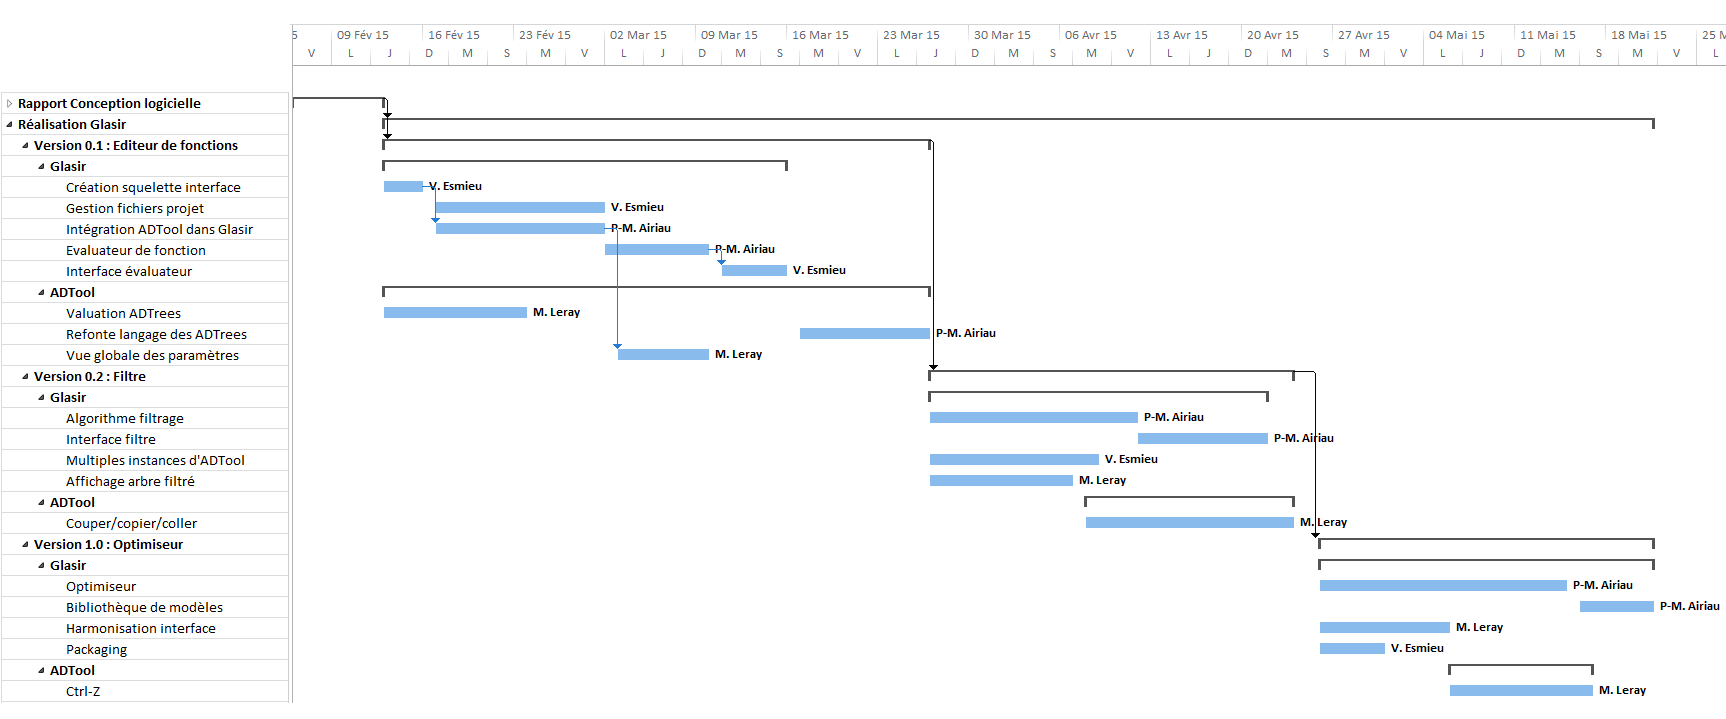
\includegraphics[height=0.66\textwidth]{figure/DiagGantt.png}
                \caption{Diagramme de Gantt présentant la chronologie des tâches.}
                \label{fig:gantt}
            \end{figure}
        \end{landscape}

        \begin{landscape}
            \begin{figure}
                \centering
                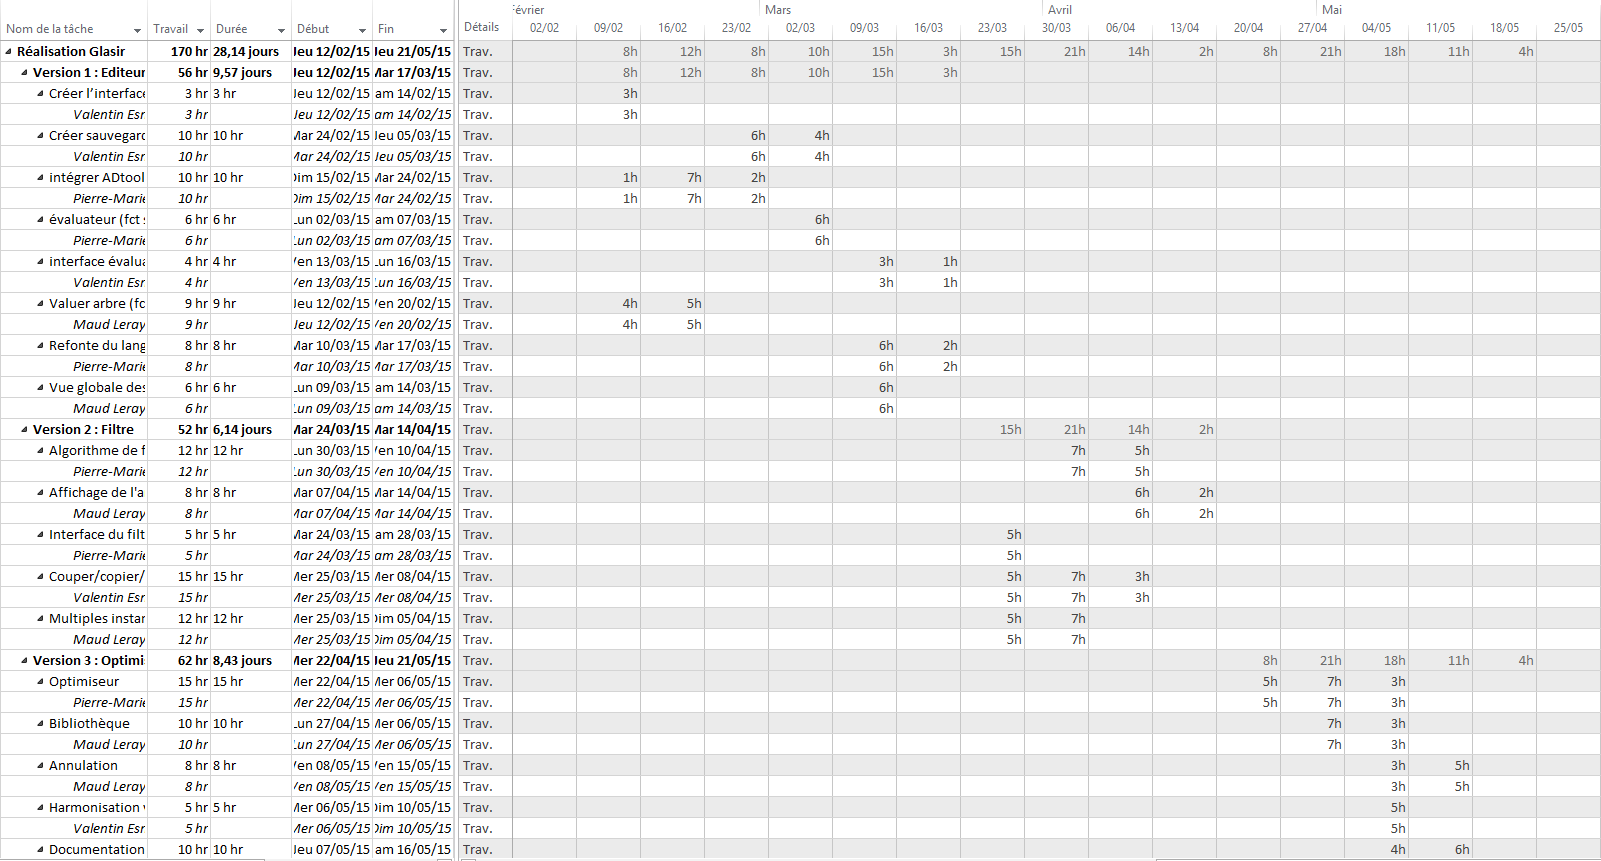
\includegraphics[height=0.66\textwidth]{figure/RepartitionTaches2.png}
                \caption{Planning des charges réparties par personne.}
                \label{fig:planning_charge}
            \end{figure}
        \end{landscape}

        \begin{landscape}
            \begin{figure}
                \centering
                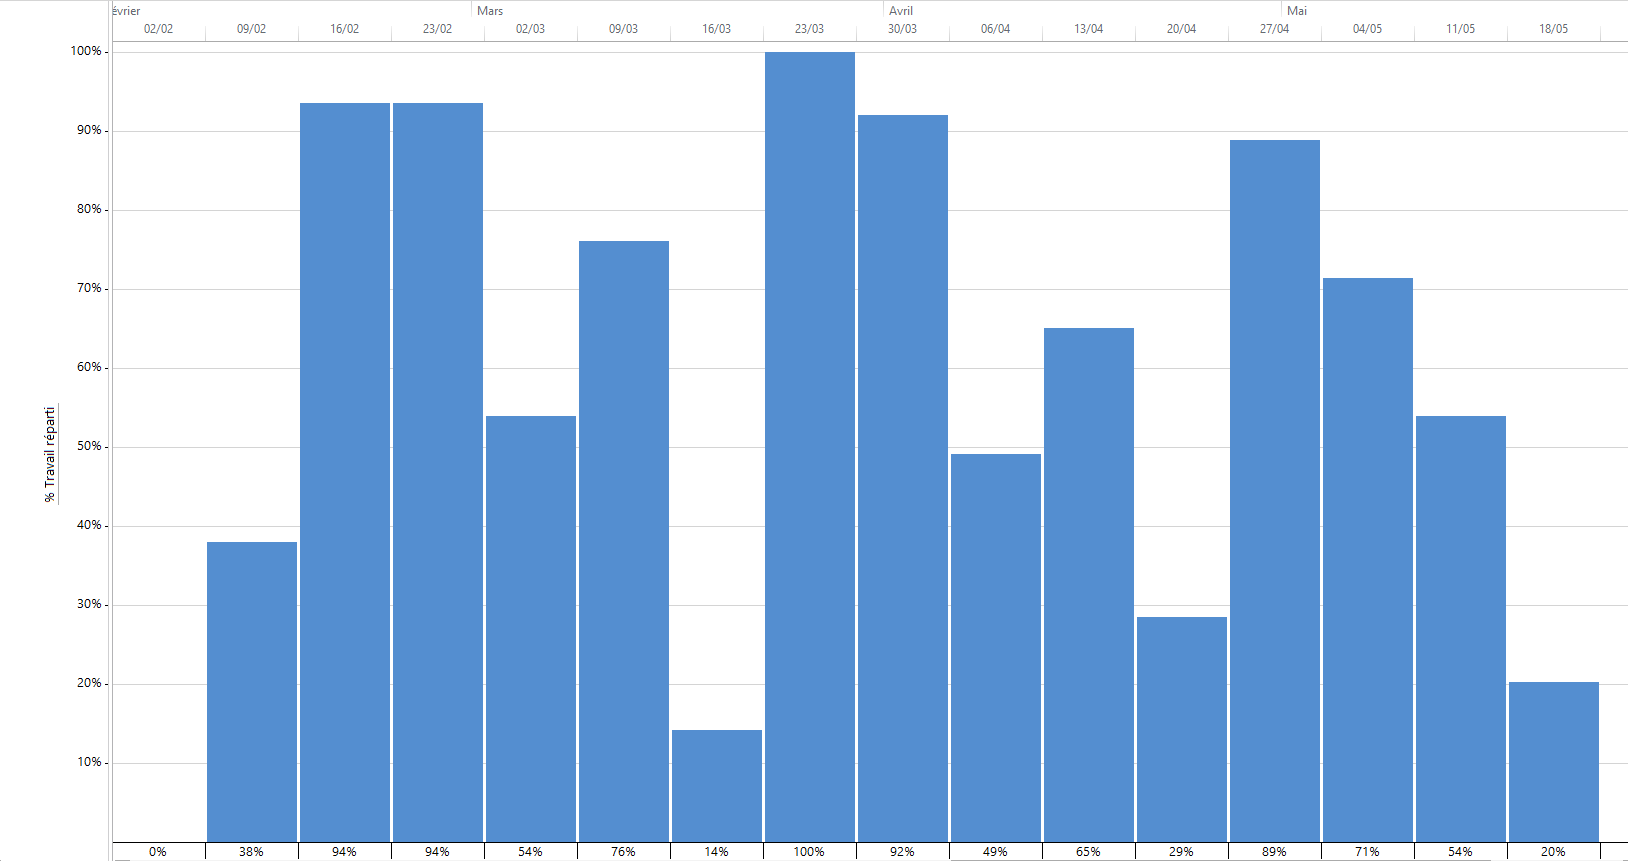
\includegraphics[height=0.70\textwidth]{figure/TauxUtilisation.png}
                \caption{Taux d'utilisation global des ressources.}
                \label{fig:taux_utilisation}
            \end{figure}
        \end{landscape}
